\chapter{Superposition, and Multipass}
\label{c:super.multi}

\index{superposition}\index{multipass}
This chapter covers two concepts: \vn{superposition} (\sref{s:super})
and \vn{multipass} (\sref{s:multipass}) \vn{Superposition} is used
when elements overlap spatially.  \vn{Multipass} is used when an
element is ``shared'' between branches such as the interaction region
shared by two storage rings, or when a beam goes through the same
physical element in a branch multiple times as in an energy recovery
linac.

In both cases, \vn{lord} and \vn{slave} elements (\sref{s:lord.slave})
are constructed by \bmad to hold the necessary information. In both
cases, the \vn{lord} elements will represent the ``physical'' element
while the \vn{slave} elements will embody the ``beam path''.

%-----------------------------------------------------------------------------
\section{Superposition}
\label{s:super}
\index{superimpose|hyperbf}

In practice the field at a particular point in the lattice may be due
to more than one physical element. One example of this is a quadrupole
magnet inside a larger solenoid magnet. \bmad has a mechanism to
handle this using what is called ``superposition''. A
simple example shows how this works:
\begin{example}
  Q: quad, l = 10
  D: drift, l = 10
  S: solenoid, l = 6, superimpose, ref = q, ref_end, offset = -1
  lat: line = (Q, D)
  use, lat
\end{example}
The \vn{superimpose} attribute of element \vn{S} superimposes \vn{S}
over the lattice \vn{(Q, D)}. The placement of \vn{S} is such that the
center of \vn{S} is offset -1~meter from the end of \vn{Q} (more on how
superimposed elements get placed later). The tracking part of the
lattice list (the part that one does tracking through) Looks like:
\begin{example}
        Element   Key         Length  Total     
  1)    Q{\#}1       Quadrupole   6        6
  2)    Q{\B}S       Sol_quad     4       10
  3)    S{\#}1       Solenoid     2       12
  4)    D{\#}2       Drift        8       20
\end{example}
What \bmad has done is to split the original elements \vn{(Q, D)} at
the edges of \vn{S}. The first element in the lattice, \vn{Q\#1}, is
the part of \vn{Q} that is outside of \vn{S}. Since this is only part
of \vn{Q}, \bmad has put a \vn{\#1} in the name so that there will be
no confusion. (\vn{\#} has no special meaning other than the fact
that \bmad uses it for mangling names). The next element, \vn{Q{\B}S},
is the part of \vn{Q} that is inside \vn{S}. \vn{Q{\B}S} is a
combination solenoid/quadrupole element as one could
expect. \vn{S{\#}1} is the part of \vn{S} that is outside \vn{Q} so
this element is just a solenoid. Finally, \vn{D\#2} is the rest of the
drift outside \vn{S}.

When \bmad sets the element class for elements created from
superpositions, \bmad will set the class of the element to something
other than an \vn{em_field} element (\sref{s:em.field}) if
possible. If no other possibilities exist, \bmad will use
\vn{em_field}. For example, a \vn{quadrupole} superimposed with a
\vn{solenoid} will produce a \vn{sol_quad} element but a \vn{solenoid}
superimposed with a \vn{rfcavity} element will produce an
\vn{em_field} element since there is no other class of element that
can simultaneously handle solenoid and RF fields.

\begin{figure}[tb]
\centering 
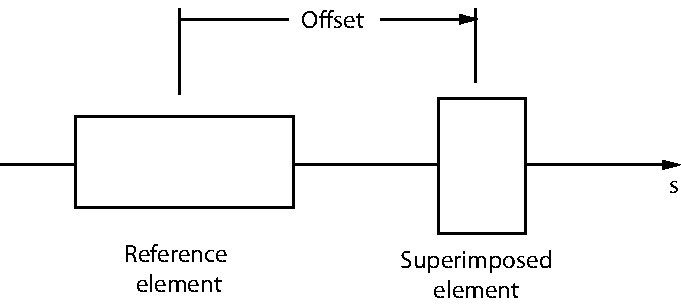
\includegraphics{superimpose.pdf} 
\caption[Superposition Illustration.]
{Illustration of a superposition.}
\label{f:superimpose}
\end{figure}

With the lattice broken up like this \bmad has constructed something
that can be easily analyzed. However, the original elements \vn{Q} and
\vn{S} still exist within the lord section of the lattice. \bmad has
bookkeeping routines so that if a change is made to the \vn{Q} or
\vn{S} elements then these changes can get propagated to the
corresponding slaves. It does not matter which element is
superimposed. Thus, in the above example, \vn{S} could have been put
in the Beam Line (with a drift before it) and \vn{Q} could then have
been superimposed on top and the result would have been the same
(except that the split elements could have different names).

If a zero length element, such as a marker, is superimposed with some
other element (or vice versa) the element is just split in two. For
example:
\begin{example}
  Q: quad, l = 10
  M: marker, superimpose, offset = 6
  lat: line = (Q)
  use, lat
\end{example}
The resulting is that the tracking part of the lattice would be
\begin{example}
        Element   Key           Length
  1)    Q{\#}1       Quadrupole    6
  2)    M         Marker        0
  3)    Q{\#}2       Quadrupole    4
\end{example}
and the lord part of the lattice would have the \vn{Q} element.
 
A superposition is illustrated in \fig{f:superimpose} The
placement of a superimposed element is determined by three factors: A
reference point on the superimposed element, a reference point in the
lattice line, and an offset between the points. The attributes that
determine these three quantities are: 
\index{ref}\index{offset}
\index{ref_beginning}\index{ref_center}\index{ref_end}
\index{ele_beginning}\index{ele_center}\index{ele_end}
\begin{example}
  create_em_field_slave = <Logical>
  ref                   = <element name in lattice>
  offset                = <length>      ! default = 0
  ele_beginning
  ele_center                            ! default
  ele_end
  ref_beginning
  ref_center                            ! default
  ref_end
\end{example}
\vn{ref} sets the reference element. If \vn{ref} is not present then
the start of the lattice is used. \vn{ref_beginning}, \vn{ref_center}
or \vn{ref_end} can be used to indicate where on the reference element
the reference point is. Default is \vn{ref_center}. Similarly,
\vn{ele_beginning}, \vn{ele_center}, or \vn{ele_end} can be used to
indicate the reference point on the superimposed element at the
beginning (entrance) edge, the center, or the end (exit) edge
respectively. If neither of these attributes are given the default is
to use the element center. \vn{offset} is the longitudinal offset
between the reference point on the reference element and the reference
point on the superimposed element. The default if not present is zero.

\index{geometry}
\index{open}
\index{drift}
\index{overlay}
\index{group}
\index{girder}
Superposition may be done with any element except \vn{Drift},
\vn{Group}, \vn{Overlay}, and \vn{Girder} control elements. A
superimposed element that extends beyond either end of the lattice
will be wrapped around so part of the element will be at the beginning
of the lattice and part of the element will be at the end. For
consistency's sake, this is done even if the \vn{geometry} is set
to \vn{open} (for example, it is sometimes convenient to
treat a circular lattice as linear). Example:
\begin{example}
  d: drift, l = 10
  q: quad, l = 2, superimpose
  machine: line = (d)
  use, machine
\end{example}
The lattice will have three elements in the tracking section:
\begin{example}
        Element   Key           Length
  3)    Q{\#}2       Quadrupole    1
  2)    D{\#}1       Drift         8
  1)    Q{\#}1       Quadrupole    1
\end{example}
The lord section of the lattice will have the element \vn{Q}. 

\index{drift!superposition}\index{pipe!superposition}
When a superposition is made that overlaps a drift the drift, not
being a "real" element, vanishes. That is, it does not get put in the
lord section of the lattice.  Note that if aperture limits
(\sref{s:limit}) have been assigned to a drift, the aperture limits
can ``disappear'' when the superposition is done. Explicitly, if the
exit end of a drift has been assigned aperture limits, the limits will
disappear if the superimposed element overlays the exit end of the
drift. A similar situation applies to the entrance end of a drift. If
this is not desired, use a \vn{pipe} element instead.

When the attributes of a super_slave are computed from the attributes
of its super_lords, some types of attributes may be ``missing''. For
example, it is, in general, not possible to set appropriate aperture
attributes (\sref{s:limit}) of a super_slave if the lords of the slave
have differing aperture settings. When doing calculations, \bmad will
use directly the corresponding attributes stored in the lord elements to
correctly calculate things.

%-----------------------------------------------------------------------------
\subsection{em_field_slave}
\label{s:super.field}



%-----------------------------------------------------------------------------
\subsection{Changing Element Lengths when there is Superposition}
\label{s:super.length}

\index{overlay}
\index{group}
\index{expand_lattice}
When the lattice is constructed, superposition of elements is done
before the addition of any \vn{group} or \vn{overlay} elements. This
is done since \vn{overlay}s and \vn{group}s are allowed to refer
to elements that are superimposed. This can lead to some unexpected
results. For example:
\begin{example}
  q1: quad, l = 10
  q2: quad, l = 10
  lat: line = (q1, q2)
  use, lat
  o: overlay = \{q1\}, l = 12
  m: marker, superimpose, offset = 15
\end{example} 
In this example, the marker is initially positioned at 15~meters from
the beginning of the lattice.  The application of the overlay will
increase the length of \vn{q1} by 2~meters which will push the marker
\vn{m} to 17~meters which might not be what was intended. To avoid
this problem, an \vn{expand_lattice} statement (\sref{s:expand}) can
be placed after the overlay, but before the superimpose, statement
\begin{example}
  ...
  o: overlay = \{q1\}, l = 12
  expand_lattice
  m: marker, superimpose, offset = 15
\end{example} 

The length of a superimposed element must necessarily be equal to the
sum of the lengths of its slave elements. For example, the element
\vn{S} in the first example of Section~\sref{s:super} has a length of
6~meters which is equal to the sum of the length of \vn{Q{\B}S}
(3~meters) plus the length of \vn{S{\#1}} (also 3~meters).

If the length of a superimposed element is varied after the lattice
has been expanded, the length of the slaves will be adjusted
accordingly. For example, if, after lattice expansion, the length of
element \vn{S} in the first example of Section~\sref{s:super} is
increased by 50\% from 6~meters to 9~meters, the lattice would look
like
\begin{example}
        Element   Key         Length  Total
  1)    Q{\#}1       Quadrupole   4        4
  2)    Q{\B}S       Sol_quad     6       10
  3)    S{\#}1       Solenoid     3       13
  4)    D{\#}2       Drift        8       21
\end{example}
The length of \vn{Q{\B}S} has been increased by 50\% from 4~meters to
6~meters and the length of \vn{S{\#}1} has been increased by 50\% from
2~meters to 3~meters to give the proper length for \vn{S}.
Additionally, to keep the length of \vn{Q} at 10~meters, the
length of \vn{Q{\#}1} has been decreased to 4~meters. The overall
length of the lattice has increased by 1~meter.

Notice that this result is {\em not} what would be obtained if the
length of the element \vn{S} is increased to 9~meters in the lattice
file. The reason for this incompatibility stems from the fact that the
effect of varying an element's length in the lattice file depends upon
what reference points are used for specifying any superpositions. For
example, if the reference point of \vn{S} in the first example of
Section~\sref{s:super} is changed to
\begin{example}
  S: solenoid, l = 6, superimpose, ele_beginning, offset = 6
\end{example}
The expanded lattice is unaltered. But with this shifted reference
point, the effect of changing the length of \vn{S} is different. That is
\begin{example}
  S: solenoid, l = 7, superimpose, ref = q, ref_end, offset = -1
\end{example}
will not produce the same expanded lattice as
\begin{example}
  S: solenoid, l = 7, superimpose, ele_beginning, offset = 6
\end{example}
Thus if someone using a simulation program is only considering the
expanded lattice, there is the potential for confusion if length
changes mirrored the effect of changing the lengths in the lattice
file.  To avoid this, and to simplify the computational overhead,
\bmad chooses to use a relatively simple algorithm for adjusting
lengths after lattice expansion. Notice that for layout design, the
\vn{no_superimpose} command (\sref{s:debug}) can be used to
suppress superposition.

%-----------------------------------------------------------------------------
\section{Multipass}
\label{s:multipass}
\index{multipass|hyperbf}

Some lattices have the beam recirculating through the same element
multiple times. For example, an Energy Recovery Linac (ERL) will
circulate the beam back through the LINAC part to retrieve the energy
in the beam. In \bmad this situation can simulated using the
\vn{multipass} attribute. A simple example shows how this works.
\index{expand_lattice}
\begin{example}
  RF1: lcavity
  linac_part: line[multipass] = (RF1, ...)
  my_line: line = (linac_part, ..., linac_part)
  use, my_line
  expand_lattice
  RF1\B2[dphi0] = 0.5
\end{example}
The tracking part of the lattice consists of two slave elements
\begin{example}
  RF1\B1, ..., RF1\B2, ...
\end{example}
Since the two elements are derived from a \vn{multipass} line they are
given unique names by adding a \vn{{\B}n} suffix. In addition there is
a lord element (that doesn't get tracked through) called \vn{RF1} in the
lord part of the lattice. Changes to attributes of the lord \vn{RF1}
element will be passed to the slave elements by \bmad's bookkeeping
routines. Assuming \vn{RF1\B1} is an accelerating cavity, to make
\vn{RF1\B2} a decelerating cavity the \vn{dphi0} attribute of
\vn{RF1\B2} is set to 0.5. This is the one attribute that \bmad's
bookkeeping routines will not touch when transferring attribute values
from \vn{RF1} to its slaves. Notice that the \vn{dphi0} attribute had to
be set after \vn{expand_lattice} (\sref{s:expand})
is used to expand the lattice since
\bmad does immediate evaluation and \vn{RF1\B2} does not exist before
the lattice is expanded.

Sublines of a multipass line are automatically multipass:
\begin{example}
  a_line: line = (...)
  m_line: line[multipass] = (..., a_line, ...)
\end{example}
In this example \vn{a_line} is implicitly multipass.

Multiple elements of the same name in a multipass line are considered 
physically distinct:
\begin{example}
  m_line: line[multipass] = (A, A, B)
  u_line: line = (m_line, m_line)
  use, u_line
\end{example}
In this example the tracking part of the lattice is
\begin{example}
  A\B1, A\B1, B\B1, A\B2, A\B2, B\B2
\end{example}
In the control section of the lattice there will be two multipass
lords called \vn{A} and one called \vn{B}. The first \vn{A} lord 
controls the 1\St and 4\Th elements in the tracking part of the lattice 
and the second \vn{A} lord controls the 2\Nd and 5\Th elements.

%-----------------------------------------------------------------------------
\subsection{The Reference Energy in a Multipass Line}
\label{s:ref.e.multi}

\index{lcavity}
\index{p0c}\index{e_tot}\index{n_ref_pass}
If there are \vn{lcavity} elements in the lattice then the reference
energy at a given element may differ from pass to pass. In this case,
the normalized strength (k1, kick, etc.) for magnetic and electric
elements will not be the same from pass to pass. To avoid an
ambiguity, all magnetic and electric elements that are used in a
multipass line must have their magnetic or electric field strength set
as the independent attribute (\sref{s:depend}), {\em or} a reference
energy (\sref{s:energy}) must be defined. A reference energy is
defined by setting \vn{e_tot} or \vn{p0c}, or by setting
\vn{n_ref_pass} as described below. The default is for \vn{n_ref_pass}
to be set to 1.

To set the reference energy, one (and only one) of the attributes
\vn{n_ref_pass}, \vn{e_tot} or \vn{p0c} needs to be
set. \vn{n_ref_pass} is an integer indicating which pass is used to
define the reference energy for the lord element. The default if
nothing is set, is for \vn{n_ref_pass} to be set to 1.  Note: If
\vn{ref_orbit} is set to \vn{match_global_coords}, or for any element
where the reference energy is not constant (like an \vn{lcavity}),
\vn{n_ref_pass} must be used and must be set to 1.
